\documentclass[runningheads]{llncs}

\usepackage[T1]{fontenc}
\usepackage[utf8]{inputenc}
\usepackage{graphicx}
\usepackage{amsmath}
\usepackage{amsfonts}
\usepackage{booktabs}
\usepackage{multirow}
\usepackage{hyperref}
\usepackage{color}
\renewcommand\UrlFont{\color{blue}\rmfamily}

\graphicspath{{figure/}}

\begin{document}

\title{Physics-Informed Explainable Deep Learning for Disinfection By-Products Prediction}

\titlerunning{Physics-Informed Deep Learning for DBPs Prediction}

\author{Anonymous}

\authorrunning{Anonymous}

\institute{Anonymous Institution\\
\email{anonymous@anonymous.edu}}

\maketitle

\begin{abstract}
Disinfection by-products (DBPs) formed during water treatment pose significant health risks, necessitating accurate and interpretable prediction models. This study presents a comprehensive evaluation of fourteen machine learning approaches for DBPs prediction, with a focus on a novel physics-informed explainable deep learning architecture. Using a dataset of 66 water samples with eight water quality parameters and five haloacetic acid targets, we systematically compare models spanning linear regression, ensemble methods, kernel methods, neural networks, and modern tabular deep learning (TabNet). Support Vector Regression (SVR) achieved the best generalization with test R$^2$ = 0.401 and 5-fold CV R$^2$ = 0.494$\pm$0.095, while the proposed physics-informed Explainable Model achieved the lowest test MAE of 0.408 with test R$^2$ = 0.303, demonstrating that chemical domain knowledge integration offers complementary advantages beyond R$^2$ optimization. The model's attention mechanism successfully learned chemically meaningful feature group weights: organic matter (44.0\%), nitrogen compounds (32.6\%), environmental conditions (14.7\%), halides (5.9\%), and disinfectant (2.8\%). Systematic ablation studies confirmed DOC ($\Delta$R$^2$=$-$0.519) and temperature ($\Delta$R$^2$=$-$0.205) as the most critical monitoring parameters.

\keywords{disinfection by-products \and physics-informed machine learning \and explainable AI \and water treatment \and haloacetic acids \and attention mechanism}
\end{abstract}


\section{Introduction}

Chlorination remains the dominant water disinfection strategy worldwide due to its efficacy against a broad spectrum of pathogens, residual protection capability throughout distribution networks, and low operational cost~\cite{deborde2008reactions,crittenden2012mwh}. A well-documented side effect is the formation of disinfection by-products (DBPs) through reactions between chlorine and natural organic matter (NOM) present in source water. Epidemiological studies have linked long-term DBP exposure to elevated risks of bladder cancer, adverse reproductive outcomes including low birth weight and spontaneous abortion, and potential carcinogenic effects~\cite{villanueva2004disinfection,richardson2007occurrence}. In response, regulatory agencies worldwide have set maximum contaminant levels (MCLs) for key DBP classes, where the USEPA mandates an MCL of 60~$\mu$g/L for five haloacetic acids (HAA5) and 80~$\mu$g/L for four trihalomethanes (TTHM), creating a pressing operational need for reliable DBPs monitoring and prediction in water treatment facilities.

The practical challenge of DBPs monitoring is substantial. Measuring individual HAA species requires gas chromatography/mass spectrometry (GC/MS) with complex sample pre-treatment, laboratory turnaround times of 24--72 hours, and analytical costs that preclude the high-frequency sampling needed for real-time process control~\cite{li2018drinking}. Predictive models that estimate DBPs concentrations from routinely measured water quality parameters offer a cost-effective alternative, enabling water treatment operators to anticipate exceedances and adjust treatment processes proactively rather than reactively.

DBPs formation is governed by a complex network of chemical reactions spanning multiple precursor types, competing pathways, and environmental modulators. The primary pathway, in which DOC and UVA254-absorbing aromatics react with hypochlorous acid (HOCl) to form haloacetic acids, is simultaneously modulated by nitrogen compounds that competitively consume chlorine (shifting both DBP quantity and speciation), temperature-dependent reaction kinetics governed by the Arrhenius equation, pH-controlled chlorine speciation between the more reactive HOCl and less reactive OCl$^-$, and bromide ions that preferentially divert reactions toward cytotoxic brominated DBP species. These interactions are inherently non-linear and partially antagonistic, rendering empirical equations and linear regression models structurally incapable of capturing the full formation dynamics~\cite{sohn2004disinfectant}.

Machine learning has emerged as a promising framework for DBPs prediction~\cite{kulkarni2010disinfection}, demonstrating substantially improved accuracy over linear models. However, a critical gap persists: existing models prioritize predictive accuracy without mechanistic interpretability. Water treatment operators need to understand \textit{which} parameters drive DBPs formation on a given day and \textit{which} interventions would reduce risk, questions black-box models cannot answer. Post-hoc methods such as SHAP~\cite{lundberg2017unified} partially address this but lack structural guarantees that explanations reflect actual learned mechanisms. An architecture embedding chemical knowledge \textit{structurally} provides interpretability by construction.

Physics-informed machine learning~\cite{raissi2019physics} offers exactly this paradigm: domain knowledge constrains model architecture during training rather than being applied as an external explanation layer. In this work, we instantiate this paradigm for HAA prediction by designing a deep learning architecture whose computational structure directly mirrors DBPs formation chemistry. The main contributions are:
\begin{enumerate}
\item \textbf{Architecture innovation.} A physics-informed explainable architecture encoding DBPs chemistry through five chemically motivated feature groups and a group-level attention mechanism, whose learned weights serve as data-driven quantitative validators of established chemical theory.
\item \textbf{Empirical benchmark.} Systematic comparison of fourteen algorithms (linear models, ensemble methods, kernel methods, and modern tabular deep learning including TabNet and KAN), showing SVR outperforms deep learning under small-sample constraints ($n$=66).
\item \textbf{Monitoring guidance.} Ablation experiments identifying DOC and temperature as highest-priority parameters ($\Delta$R$^2$=$-$0.519 and $-$0.205) and revealing that low-variance features (e.g., Cl$_2$) degrade performance in data-scarce regimes.
\end{enumerate}


\section{Related Work}

\paragraph{Machine learning for DBPs and water quality prediction.}
Predictive modeling for DBPs has progressed through three generations. Early empirical kinetic models~\cite{sohn2004disinfectant} and multiple linear regression approaches~\cite{uyak2007multiple} provided mechanistic transparency but failed to capture the non-linear formation dynamics inherent to multi-precursor chlorination chemistry. The second generation adopted statistical learning: Kulkarni and Chellam~\cite{kulkarni2010disinfection} demonstrated that artificial neural networks substantially outperform linear models for DBPs formation prediction by capturing feature interaction effects; Hong et al.~\cite{hong2016using,hong2017bromine} extended regression models to Chinese water systems and highlighted the critical role of bromide incorporation in speciation prediction. Concurrently, ML methods have been applied across broader water quality prediction tasks, including trihalomethane formation~\cite{hong2015use}, dissolved oxygen, turbidity, and treatment efficiency optimization~\cite{sadiq2004disinfection}. A recurring finding is that ensemble tree methods and kernel-based regressors outperform neural networks when dataset sizes are limited ($n < 200$), while deep learning becomes advantageous at scale~\cite{li2018drinking}. Despite demonstrated accuracy gains, none of these approaches explicitly encodes the chemical reaction structure into model architecture, precluding the generation of mechanistically grounded explanations.

\paragraph{Post-hoc explainability and its limitations.}
The growing deployment of ML models in safety-critical infrastructure has driven demand for explainability. Post-hoc methods such as SHAP~\cite{lundberg2017unified} and similar post-hoc methods assign feature importance scores to a trained model's predictions. These methods have been applied to water quality models, providing useful qualitative insights into parameter relevance. However, post-hoc explainability has a fundamental limitation for scientific applications: importance scores are computed \textit{after} training and describe model behavior rather than learned chemical mechanisms. In small-sample, high-dimensional settings (precisely the conditions of DBPs monitoring), SHAP values can be unstable across data subsets and may reflect spurious statistical correlations rather than causal chemical relationships. Furthermore, these methods treat the model as a black box and provide no structural guarantee that the learned representations correspond to chemically meaningful quantities. Architecture-intrinsic interpretability, where domain knowledge directly shapes the computational graph, provides a stronger form of transparency: the model's internal structure \textit{is} the explanation.

\paragraph{Physics-informed and attention-based models.}
Physics-informed neural networks (PINNs)~\cite{raissi2019physics} embed physical laws as differential equation constraints in the loss function, enabling data-efficient learning in scientific domains. Our approach differs in that we encode chemical knowledge architecturally, through feature grouping and group-level attention, rather than through loss penalties. Attention mechanisms~\cite{vaswani2017attention}, originally developed for sequence modeling, have been adapted as interpretability tools across domains by learning input-group importance weights. TabNet~\cite{arik2021tabnet} applies sequential attention for tabular feature selection, achieving competitive accuracy on benchmark datasets with built-in sparsity. KAN~\cite{liu2024kan}, based on the Kolmogorov-Arnold representation theorem, replaces fixed node activations with learnable edge-wise spline functions, offering an alternative inductive bias for non-linear function approximation. Our work differs from all these in explicitly grounding the group structure in established DBPs formation chemistry, making the attention weights chemically interpretable rather than statistically derived.


\section{Methodology}

\subsection{Dataset}

The dataset comprised 66 water samples from drinking water distribution systems, each characterized by eight water quality parameters: temperature (Temp), pH, UV absorbance at 254~nm (UVA254), chlorine concentration (Cl$_2$), nitrite-nitrogen (NO$_2^-$-N), dissolved organic carbon (DOC), ammonium-nitrogen (NH$_4^+$-N), and bromide (Br$^-$). Target variables were five HAA species: DCAA, TCAA, BCAA, HAA5, and HAA9. All features were standardized using z-score normalization computed on the training set. The dataset was split 70\%/30\% (training: $n$=46, test: $n$=20) with random seed 42.

\subsection{Physics-Informed Explainable Model}

The core contribution is a physics-informed explainable deep learning model that embeds established DBPs formation chemistry into its computational architecture. The fundamental reaction pathway follows: \textit{Organic Precursors + HOCl/OCl$^-$ $\rightarrow$ Intermediate Products $\rightarrow$ DBPs}. The overall architecture is illustrated in Fig.~\ref{fig:arch}.

\begin{figure}[t]
\centering
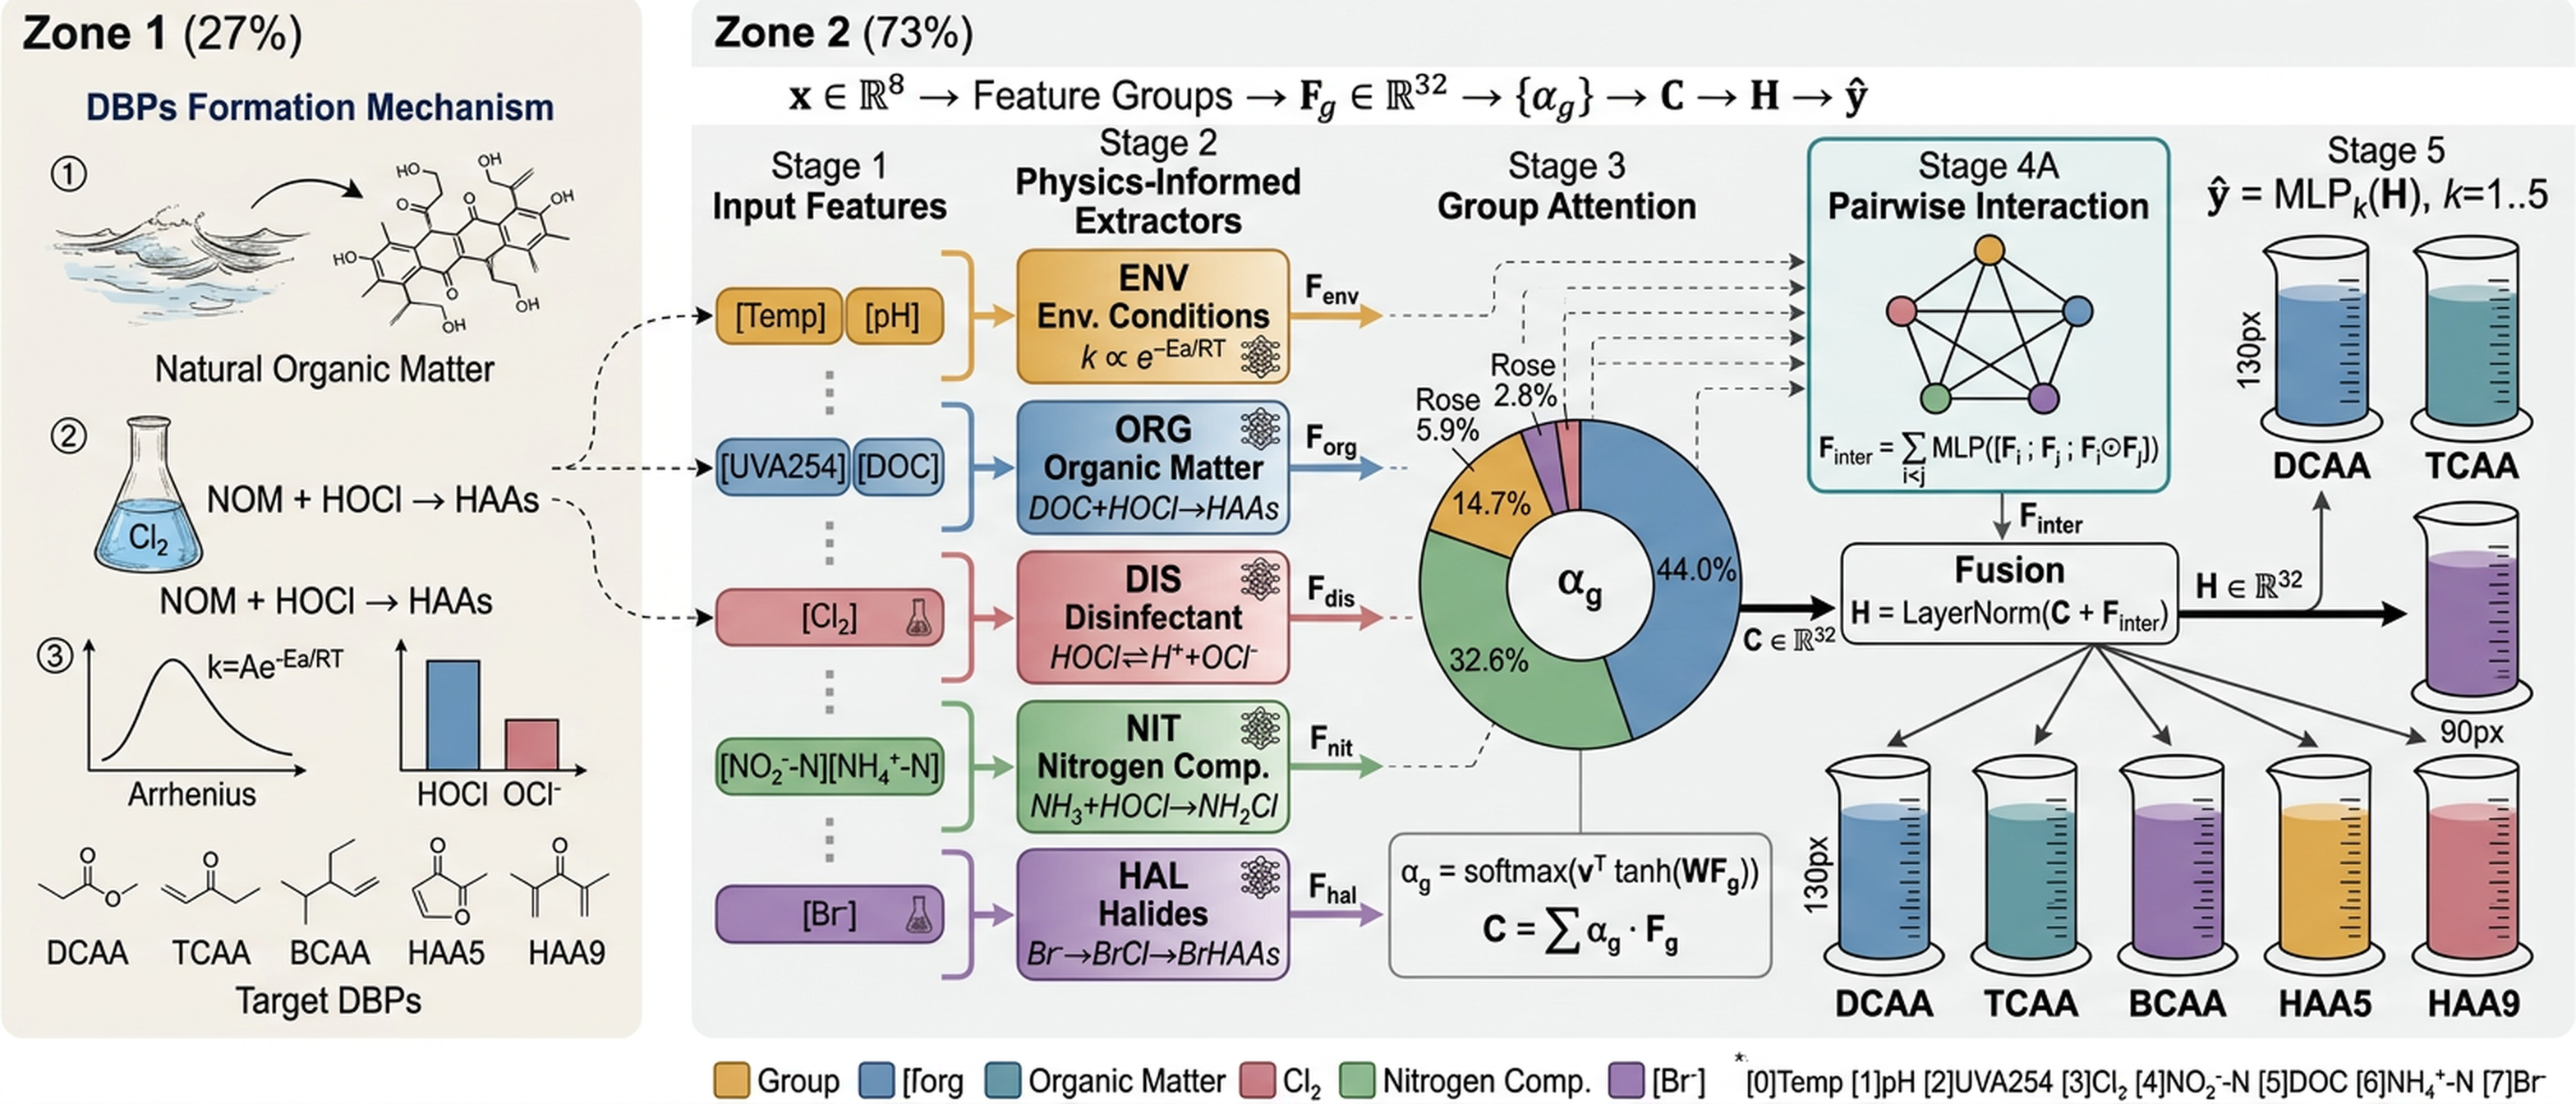
\includegraphics[width=\textwidth]{architecture.png}
\caption{Architecture of the physics-informed explainable model. Input features are partitioned into five chemically motivated groups, each processed by a dedicated MLP extractor. An attention mechanism learns group-level importance weights ($\alpha_g$), a pairwise interaction module captures inter-group synergies, and five task-specific branches predict individual HAA species simultaneously.}
\label{fig:arch}
\end{figure}

\textbf{Physics-informed feature grouping.} Rather than treating all features equivalently, the model partitions the input space $\mathbf{X} \in \mathbb{R}^{n \times 8}$ into five chemically meaningful groups reflecting distinct physicochemical processes:
\begin{itemize}
  \item \textit{Environmental conditions} $\{T, \text{pH}\}$: control reaction kinetics via Arrhenius law and chlorine speciation (HOCl $\rightleftharpoons$ H$^+$ + OCl$^-$)
  \item \textit{Organic matter} $\{\text{UVA254}, \text{DOC}\}$: quantify precursor reactivity and aromatic content
  \item \textit{Disinfectant} $\{\text{Cl}_2\}$: primary oxidizing agent
  \item \textit{Nitrogen compounds} $\{\text{NO}_2^--\text{N}, \text{NH}_4^+-\text{N}\}$: competitive chlorine consumers
  \item \textit{Halides} $\{\text{Br}^-\}$: control brominated DBPs formation
\end{itemize}
Each group is processed by a dedicated MLP feature extractor:
\begin{equation}
\mathbf{F}_g = \text{MLP}_g(\mathbf{x}_g) = \mathbf{W}_g^{(3)} \sigma(\mathbf{W}_g^{(2)} \sigma(\mathbf{W}_g^{(1)} \mathbf{x}_g + \mathbf{b}_g^{(1)}) + \mathbf{b}_g^{(2)}) + \mathbf{b}_g^{(3)}
\end{equation}

\textbf{Attention-based chemical weighting.} An attention mechanism learns the relative importance of each chemical process group:
\begin{equation}
e_g = \mathbf{v}_{att}^T \tanh(\mathbf{W}_{att} \mathbf{F}_g + \mathbf{b}_{att}), \quad
\alpha_g = \frac{\exp(e_g)}{\sum_{j=1}^{5}\exp(e_j)}, \quad
\mathbf{C} = \sum_{g=1}^{5} \alpha_g \mathbf{F}_g
\end{equation}
The weights $\alpha_g$ provide chemically interpretable importance scores that can be validated against established chemical theory.

\textbf{Chemical interaction modeling.} Pairwise inter-group interactions capture known synergies (e.g., pH-dependent chlorine reactivity):
\begin{equation}
\mathbf{I}_{ij} = \text{MLP}_{inter}([\mathbf{F}_i;\mathbf{F}_j;\mathbf{F}_i \odot \mathbf{F}_j;|\mathbf{F}_i - \mathbf{F}_j|]), \quad
\mathbf{F}_{inter} = \sum_{i<j} \mathbf{I}_{ij}
\end{equation}

\textbf{Multi-task prediction.} Five compound-specific output branches reflect the chemical reality that different HAAs form via distinct mechanisms:
\begin{equation}
y_{\text{DBP}} = \text{MLP}_{\text{DBP}}(\text{LayerNorm}(\mathbf{C} + \mathbf{F}_{inter}))
\end{equation}

\subsection{Baseline Models}

Fourteen baseline and comparison models were implemented across five families. \textit{Linear models} (Linear Regression, Ridge, Lasso, Elastic Net) establish lower-bound performance and test whether linear relationships in the data suffice. \textit{Ensemble methods} (Random Forest~\cite{breiman2001random}, Extra Trees, Gradient Boosting, Decision Tree) represent the current state-of-the-art for tabular data but are susceptible to overfitting on small datasets due to their high effective capacity. \textit{Kernel and instance methods} (SVR with RBF kernel and K-Nearest Neighbors) were included because kernel methods are known to generalize well in high-dimensional, small-sample regimes through implicit regularization via structural risk minimization~\cite{vapnik1998statistical}; SVR with RBF kernel was specifically chosen for its non-parametric flexibility and robustness to noisy features. Modern tabular deep learning baselines include TabNet~\cite{arik2021tabnet}, which uses sequential attention for feature selection, and KAN~\cite{liu2024kan}, which replaces fixed activations with learnable spline functions on edges. Together, these fourteen baselines span the current algorithmic landscape and provide a comprehensive reference for positioning the proposed Explainable Model.

\subsection{Ablation Study Design}

The ablation study was conducted within the Explainable Model framework (rather than SVR) because only the structured architecture supports controlled feature removal within chemically defined groups. Nine configurations were evaluated: a baseline (all eight features) and eight single-feature exclusion experiments, each holding architecture, training protocol (300 epochs, identical LR schedule), and data partition (same seed 42 split) constant. Performance impact is quantified as $\Delta$R$^2$ = R$^2_{\text{removed}}$ $-$ R$^2_{\text{baseline}}$; negative values indicate degradation. Single-feature removal was chosen over group-level removal to isolate individual sensor contributions, directly informing monitoring system design.

\subsection{Training Details}

\textit{Deep learning models.} The Explainable Model was implemented in PyTorch and trained for 300 epochs with Adam ($\eta$=0.001, weight decay=$10^{-5}$), ReduceLROnPlateau scheduling (factor 0.5, patience 50), hidden dimension 32, dropout 0.2, and batch size 4. The baseline MLP used identical settings with hidden dimension 10. All hyperparameters were chosen to minimize overfitting risk given the small training set ($n$=46): batch size 4 maximizes gradient diversity, hidden dimension 32 was the largest that did not increase training-test gap, and learning rate scheduling prevents premature convergence to local minima. \textit{Classical models} used scikit-learn defaults: SVR (RBF kernel, C=1.0, $\varepsilon$=0.1), Random Forest and Gradient Boosting (100 estimators), Ridge ($\alpha$=1.0). Default hyperparameters were retained to avoid overfitting to the small validation set. All experiments used random seed 42.


\section{Results}

\subsection{Overall Model Performance}

Table~\ref{tab:model_performance} presents the comprehensive performance comparison. SVR achieved the best test R$^2$ of 0.401 with the smallest train-test gap (0.393), demonstrating superior generalization in the small-sample regime ($n$=66). TabNet ranked second (test R$^2$=0.323), while the Explainable Model achieved test R$^2$=0.303 with the best test MAE of 0.408 across all models.

Ensemble methods (Extra Trees, Random Forest, Gradient Boosting) exhibited severe overfitting with training R$^2$=1.0 but substantially lower test performance, highlighting the challenge of tree-based methods with limited data. Linear models (test R$^2 < 0.08$) confirm that DBPs formation involves substantial non-linear interactions. Figure~\ref{fig:model_comparison} visualizes the performance hierarchy across all metrics.

\begin{table}[t]
\caption{Model performance comparison (ranked by Test R$^2$). Bold: best (highest R$^2$, lowest MSE/MAE) per column.}
\label{tab:model_performance}
\centering
\footnotesize
\begin{tabular}{lrrrr}
\toprule
\textbf{Model} & \textbf{Train R$^2$} & \textbf{Test R$^2$} & \textbf{Test MSE} & \textbf{Test MAE} \\
\midrule
Support Vector Regression & 0.794 & \textbf{0.401} & \textbf{0.463} & 0.454 \\
TabNet                    & 0.738 & 0.323 & 0.512 & 0.487 \\
Explainable Model         & 0.992 & 0.303 & 0.560 & \textbf{0.408} \\
Extra Trees               & 1.000 & 0.294 & 0.540 & 0.484 \\
Neural Network            & 0.996 & 0.289 & 0.561 & 0.530 \\
Random Forest             & 0.920 & 0.228 & 0.584 & 0.504 \\
Gradient Boosting         & 1.000 & 0.200 & 0.608 & 0.483 \\
K-Nearest Neighbors       & 0.635 & 0.185 & 0.595 & 0.558 \\
KAN Model                 & 0.731 & 0.109 & 0.687 & 0.607 \\
Elastic Net               & 0.576 & 0.071 & 0.675 & 0.654 \\
Lasso Regression          & 0.530 & 0.026 & 0.704 & 0.651 \\
Ridge Regression          & 0.613 & 0.009 & 0.736 & 0.702 \\
Linear Regression         & 0.614 & $-$0.029 & 0.769 & 0.718 \\
Decision Tree             & 1.000 & $-$0.044 & 0.798 & 0.559 \\
\bottomrule
\end{tabular}
\end{table}

\begin{figure}[t]
\centering
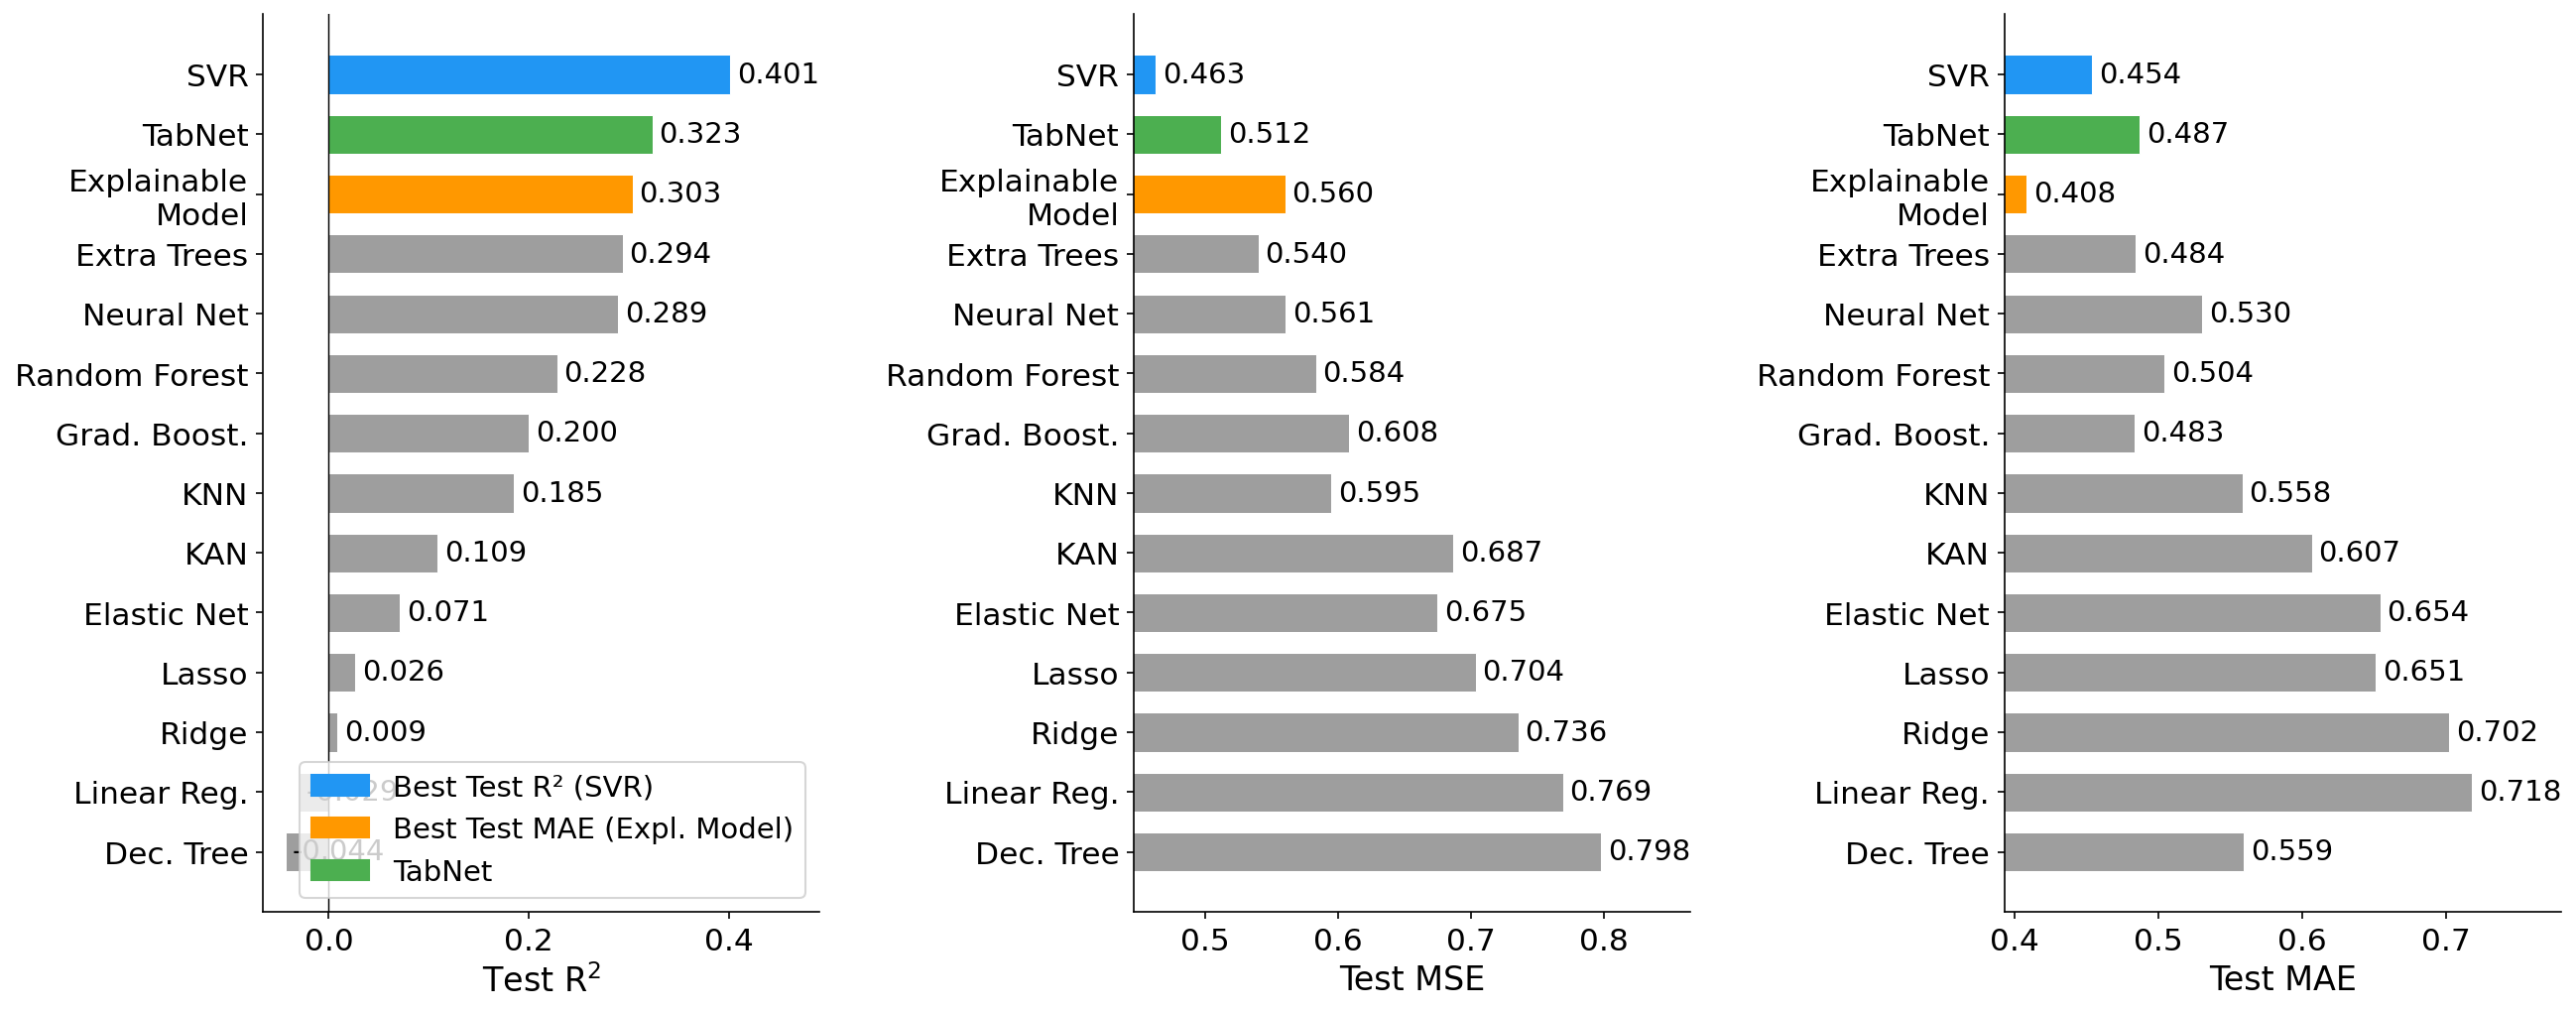
\includegraphics[width=0.95\textwidth]{model_comparison.png}
\caption{Model performance comparison across all fourteen models. SVR achieves the highest test R$^2$ while the Explainable Model achieves the lowest test MAE.}
\label{fig:model_comparison}
\end{figure}

\subsection{Explainable Model: Attention Weights and Training Dynamics}

The Explainable Model's training dynamics are shown in Fig.~\ref{fig:training_curves}. The model converges stably over 300 epochs, with the ReduceLROnPlateau scheduler effectively controlling overfitting.

The learned attention weights provide chemically interpretable feature group importance, visualized in Fig.~\ref{fig:attention}: organic matter (44.0\%), nitrogen compounds (32.6\%), environmental conditions (14.7\%), halides (5.9\%), and disinfectant (2.8\%). These weights are strongly consistent with established DBPs formation chemistry: (1) the dominance of organic matter validates DOC and UVA254 as primary precursors for haloacetic acid formation; (2) the high weight for nitrogen compounds reflects competitive chlorine consumption by NH$_3$ and NO$_2^-$; (3) the low disinfectant weight correctly reflects that Cl$_2$ dosing is typically controlled within narrow operational ranges, limiting its predictive variance. The correspondence between learned weights and chemical theory provides a form of post-hoc validation for the model architecture.

\begin{figure}[t]
\centering
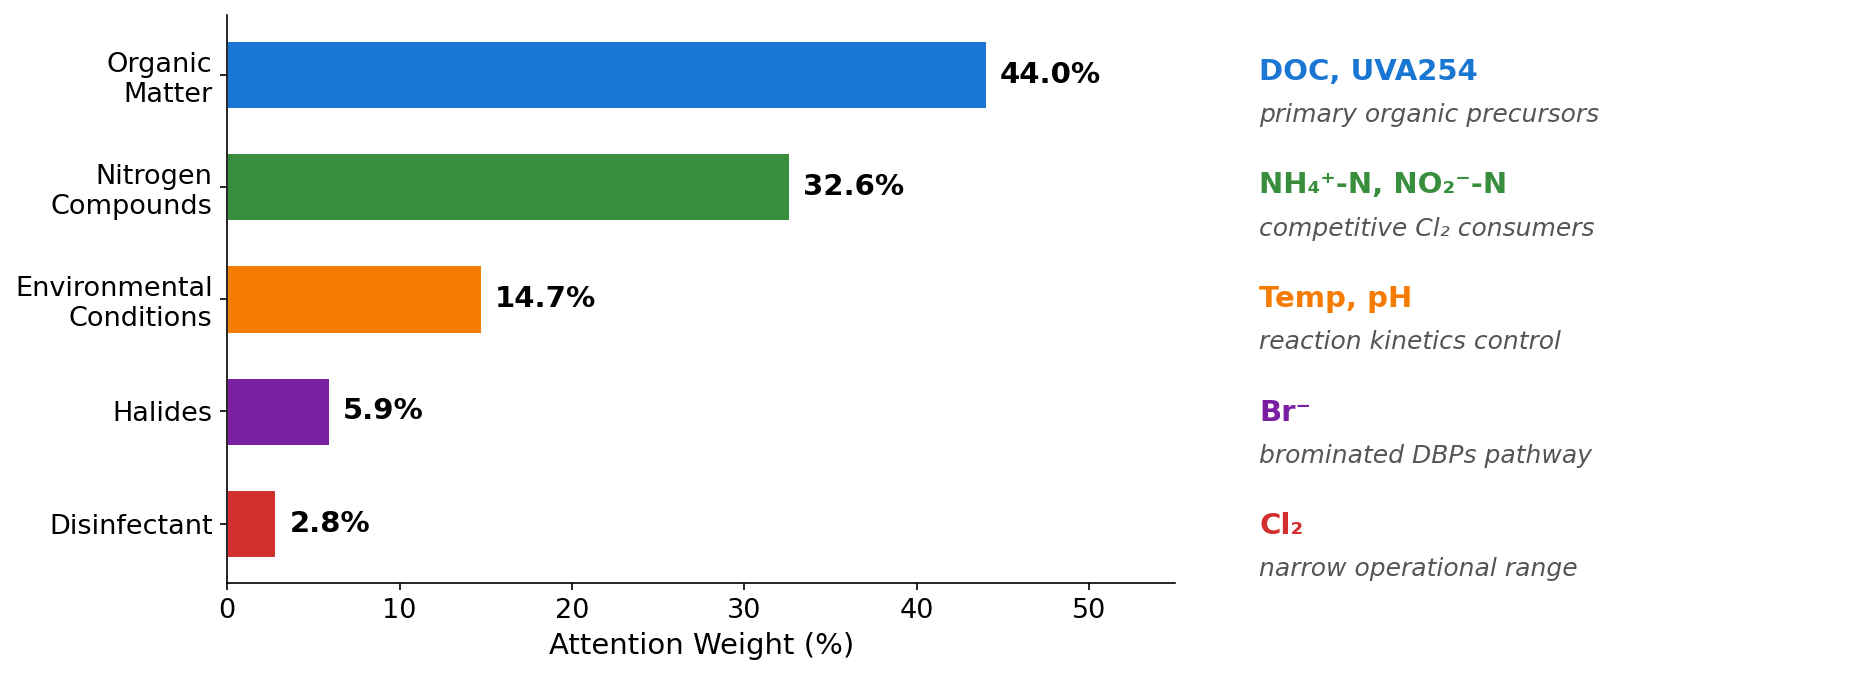
\includegraphics[width=0.85\textwidth]{attention_weights.png}
\caption{Learned attention weights for the five chemical feature groups, with chemical interpretation of each group's role in DBPs formation. Organic matter and nitrogen compounds dominate, consistent with established haloacetic acid formation mechanisms.}
\label{fig:attention}
\end{figure}

\begin{figure}[t]
\centering
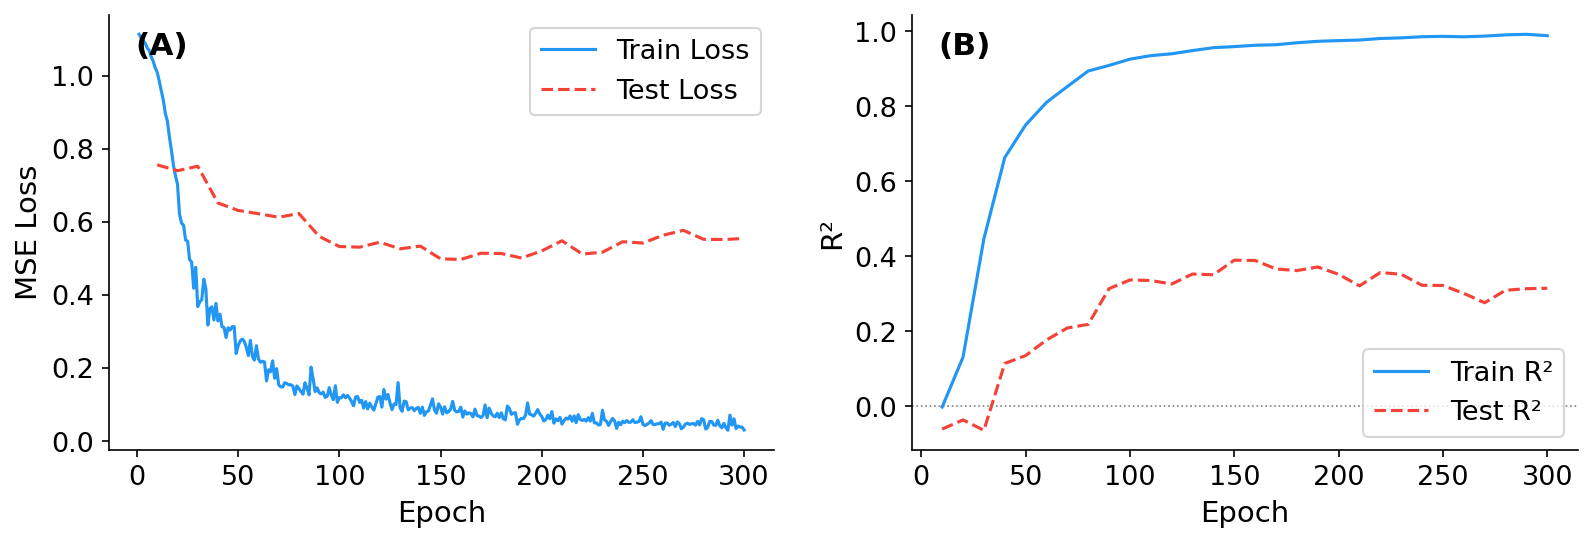
\includegraphics[width=0.9\textwidth]{training_curve.png}
\caption{Explainable Model training dynamics over 300 epochs: (A) MSE loss curves showing stable convergence, (B) R$^2$ evolution for training and test sets.}
\label{fig:training_curves}
\end{figure}

\subsection{Ablation Study: Feature Criticality}

Table~\ref{tab:ablation_results} presents the systematic ablation results (baseline test R$^2$=0.156). DOC removal caused the most severe degradation ($\Delta$R$^2$=$-$0.519, test R$^2$=$-$0.362), confirming dissolved organic carbon as the dominant precursor in HAA formation. Temperature removal produced the second-largest degradation ($\Delta$R$^2$=$-$0.205), consistent with Arrhenius-law thermodynamic control of chlorination kinetics.

Counterintuitively, removing Cl$_2$ ($\Delta$R$^2$=+0.189), NO$_2^-$-N ($\Delta$R$^2$=+0.160), Br$^-$ ($\Delta$R$^2$=+0.087), and UVA254 ($\Delta$R$^2$=+0.032) \textit{improved} test performance. This is best interpreted as a small-sample overfitting effect: features with low operational variance (particularly Cl$_2$, which is tightly controlled at water treatment facilities) contribute noise rather than useful signal in a 66-sample regime. These findings have practical implications for monitoring system design; a minimal sensor set focused on DOC and temperature may outperform comprehensive arrays under data-scarce conditions.

\begin{table}[t]
\caption{Ablation study results. $\Delta$R$^2$ = Test R$^2$ (removed) $-$ Baseline (0.156); negative values indicate performance drop.}
\label{tab:ablation_results}
\centering
\footnotesize
\begin{tabular}{lrrrr}
\toprule
\textbf{Removed Feature} & \textbf{Train R$^2$} & \textbf{Test R$^2$} & \textbf{Test MAE} & \boldmath{$\Delta$}\textbf{R$^2$} \\
\midrule
None (Baseline) & 0.930 & 0.156 & 0.501 & 0.000 \\
\midrule
Cl$_2$ (mg/L)           & 0.945 & 0.345 & 0.409 & $+$0.189 \\
NO$_2^-$-N (mg/L)       & 0.953 & 0.316 & 0.454 & $+$0.160 \\
Br$^-$ ($\mu$g/L)       & 0.955 & 0.243 & 0.474 & $+$0.087 \\
UVA254 (cm)             & 0.923 & 0.189 & 0.474 & $+$0.032 \\
pH                      & 0.937 & 0.126 & 0.540 & $-$0.030 \\
NH$_4^+$-N ($\mu$g/L)   & 0.870 & 0.063 & 0.590 & $-$0.093 \\
Temperature             & 0.960 & $-$0.048 & 0.587 & $-$0.205 \\
DOC (mg/L)              & 0.824 & $-$0.362 & 0.770 & $-$0.519 \\
\bottomrule
\end{tabular}
\end{table}

\subsection{Feature Importance and Model Correlations}

Feature importance analysis from Random Forest and Extra Trees consistently ranked DOC (RF: 0.389, ET: 0.282) and UVA254 (RF: 0.288, ET: 0.342) as the top two predictors, converging with the ablation results and the Explainable Model's attention weights to provide three independent lines of evidence for organic matter dominance. Br$^-$ (0.081--0.086) ranked third, reflecting its role in brominated DBP formation. Pearson correlation analysis among model predictions revealed three distinct algorithmic clusters: high-correlation linear models (r$>$0.94), moderate-correlation ensemble methods (0.81--0.95), and lower-correlation approaches (Explainable Model, KAN; r$<$0.75), indicating that the latter capture prediction patterns complementary to mainstream approaches, a property potentially valuable for ensemble combination strategies.

\subsection{Cross-Validation Performance}

5-fold cross-validation on the ten classical ML models provides more reliable generalization estimates than the single 70/30 split for a dataset of this size. SVR again ranks first (CV R$^2$=0.494$\pm$0.095), with Extra Trees second (0.475$\pm$0.111) and Random Forest third (0.426$\pm$0.084), consistent with single-split rankings, reinforcing the robustness of these conclusions. Decision Tree's CV R$^2$=$-$0.213$\pm$0.383 confirms severe and unstable overfitting. Deep learning models were excluded from CV due to the computational cost of 300-epoch training per fold; their generalization is assessed via the holdout test set.


\section{Discussion}

\paragraph{Kernel methods outperform deep learning under small-sample constraints.}
SVR's superiority (test R$^2$=0.401, CV R$^2$=0.494$\pm$0.095) is theoretically grounded: the maximum margin formulation minimizes structural risk regardless of dataset size, providing generalization guarantees that capacity-rich models cannot match when $n \ll d_{eff}$ (Extra Trees: Train R$^2$=1.0, Test R$^2$=0.294; Neural Network: Train R$^2$=0.996, Test R$^2$=0.289). This carries direct practical guidance: for DBPs monitoring datasets smaller than $\sim$100 samples (a common constraint given the analytical cost of HAA measurement), SVR should be the default baseline, with deep learning reserved for larger-scale deployments. Prior DBPs neural network studies reporting R$^2>0.8$~\cite{li2018drinking} consistently used larger datasets; our results are consistent with a 5$\times$ smaller training set and reflect data constraints rather than model limitations.

\paragraph{Attention weights as emergent chemical validators.}
The learned attention weights (organic matter 44.0\%, nitrogen 32.6\%, environmental 14.7\%, halides 5.9\%, disinfectant 2.8\%) emerged from data without being engineered to match chemical theory. Their agreement with established chemistry (DOC/UVA254 as primary precursors~\cite{reckhow1990chlorination}, nitrogen compounds as competitive chlorine consumers, low Cl$_2$ weight reflecting tight operational control) was not constrained during training. This represents a new use case for physics-informed ML: using learned model parameters as \textit{quantitative evidence} for chemical hypotheses, bridging data-driven and mechanistic modeling paradigms.

\paragraph{Architecture-intrinsic interpretability and monitoring implications.}
A key distinction from common XAI practice is that our interpretability is \textit{architectural}: attention weights are part of the forward pass and directly influence predictions, so the model \textit{commits} to its chemical groupings during learning rather than rationalizing them post-hoc via SHAP~\cite{lundberg2017unified} or similar explanation methods. The practical consequence is that physics-informed constraints reshape the error distribution: the Explainable Model achieves the best test MAE (0.408) despite lower R$^2$ than SVR, reducing extreme prediction failures at the cost of aggregate variance explanation. For water safety management, where large under-predictions carry greater risk than over-predictions, minimizing MAE may be operationally more relevant than maximizing R$^2$. The ablation study further reveals that DOC removal ($\Delta$R$^2$=$-$0.519) and temperature removal ($-$0.205) cause by far the largest degradation, while removing Cl$_2$ (+0.189) \textit{improves} performance, because Cl$_2$ dosing is tightly controlled at most facilities and contributes overfitting noise rather than predictive signal. For utilities with limited sensor budgets, a minimal DOC + temperature monitoring system may outperform a comprehensive eight-parameter array in data-scarce regimes.

\paragraph{Limitations and future directions.}
The primary limitation is dataset size ($n$=66), which constrains statistical power: the Wilcoxon test minimum achievable p-value with 5-fold CV is 0.0625, precluding significance claims. Results should be validated on larger, geographically diverse datasets. The focus on HAAs excludes trihalomethanes, haloacetonitriles, and emerging DBPs whose formation mechanisms differ, potentially yielding different attention weight distributions. The static snapshot dataset cannot capture seasonal dynamics or long-term trend effects. Future work should integrate temporal modeling (e.g., LSTM layers within the group extractors), explore transfer learning from data-rich systems to data-scarce ones, and extend the chemical grouping architecture to other classes of water quality predictions where domain knowledge can similarly constrain model structure.


\section{Conclusion}

We presented a physics-informed explainable deep learning architecture for HAA prediction that embeds DBPs formation chemistry through five feature groups and a group-level attention mechanism. Across fourteen algorithms, SVR achieves the best generalization (test R$^2$=0.401); the Explainable Model achieves the best test MAE (0.408) with chemically validated attention weights. Ablation studies identify DOC ($\Delta$R$^2$=$-$0.519) and temperature ($-$0.205) as highest-priority monitoring parameters. The learned attention weights, emerging from data without engineering to match theory, position physics-informed ML as a tool for scientific hypothesis testing, not just prediction. Future work should extend to larger datasets, temporal modeling, and broader DBPs families.


\bibliographystyle{splncs04}
\bibliography{references}

\end{document}
